\documentclass[12pt, letterpaper]{article}
\usepackage[utf8]{inputenc}
\usepackage[spanish,es-noquoting]{babel}
\usepackage{amsmath, amssymb, amsthm, bm}
\usepackage{graphicx}
\usepackage{array}
\usepackage{hyperref}
\usepackage{enumitem}
\usepackage{float}
\usepackage{xcolor}
\usepackage{booktabs}
\usepackage{tikz}
\usetikzlibrary{automata, positioning, arrows.meta}
\definecolor{lightgray}{rgb}{0.95,0.95,0.95}
%% Sets page size and margins
\usepackage[top=2.5cm,bottom=2.5cm,left=2cm,right=2cm]{geometry}
\usepackage{setspace}
\onehalfspacing
\usepackage{gensymb}
\usepackage{fancyhdr}
\pagestyle{fancy}
\fancyhead[L]{Compiladores}
\fancyhead[C]{Tarea 1}
\fancyhead[R]{Facultad de Ciencias UNAM}
\fancyfoot[C]{\thepage}
\renewcommand{\headrulewidth}{0.4pt}
\renewcommand{\footrulewidth}{0.4pt}

\begin{document}
\begin{titlepage}
    \centering
    \vspace{2cm}
    {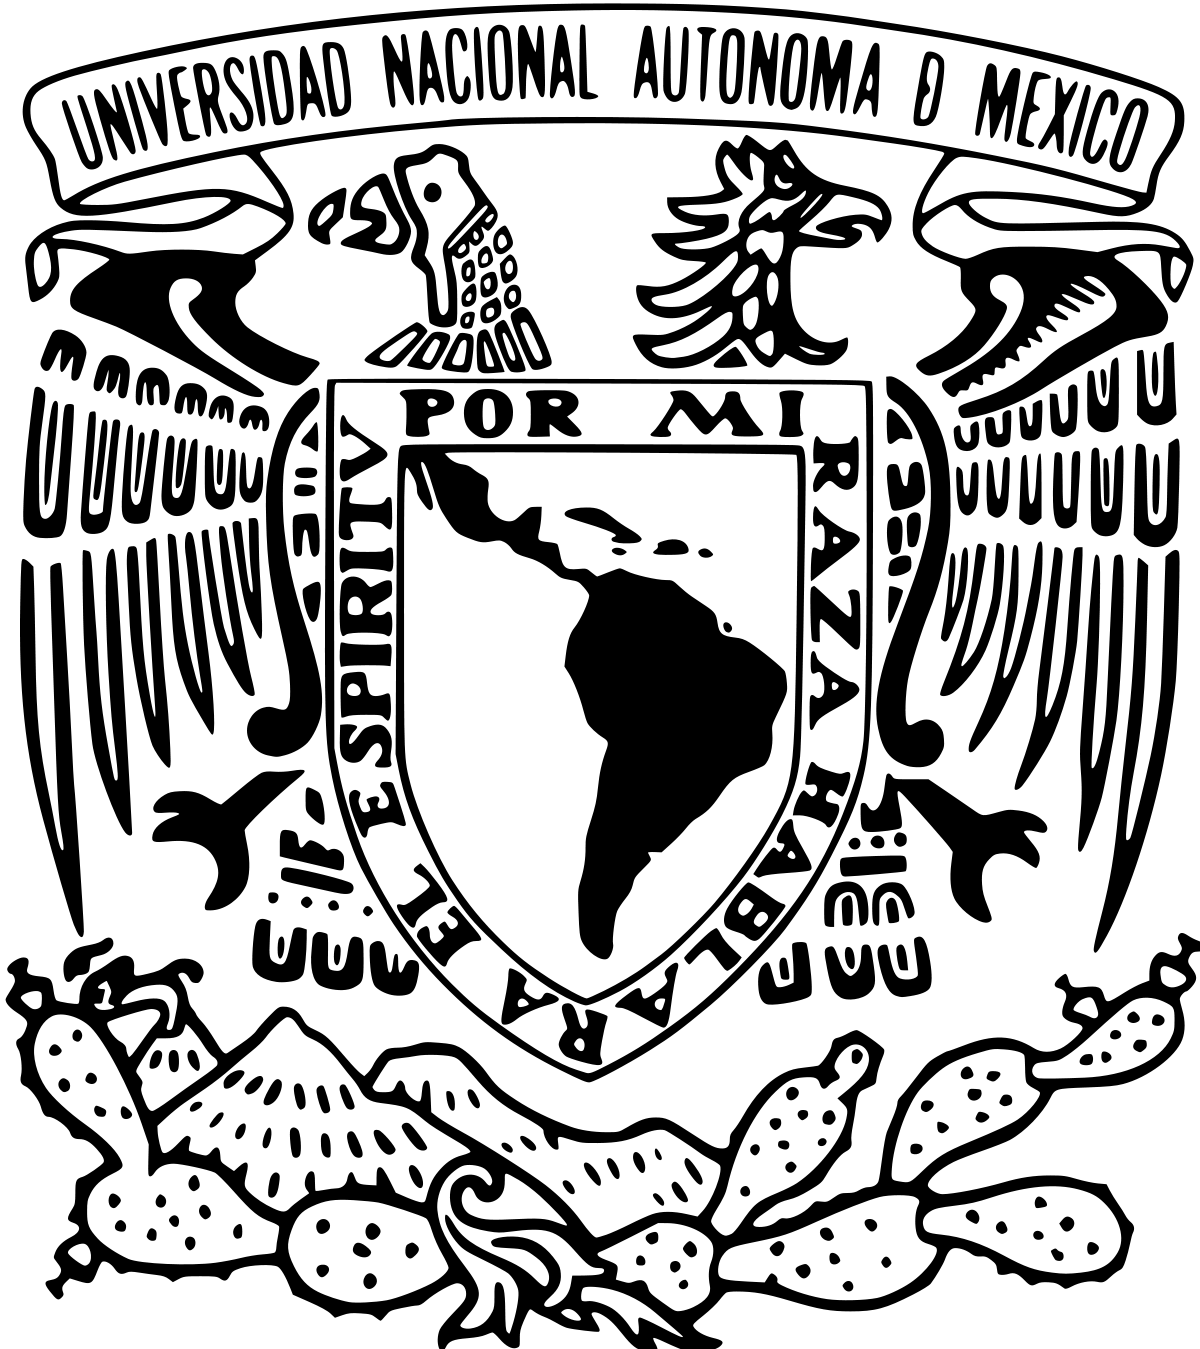
\includegraphics[height=3.2cm]{images/Logo_UNAM.png}}
    \hfill
    {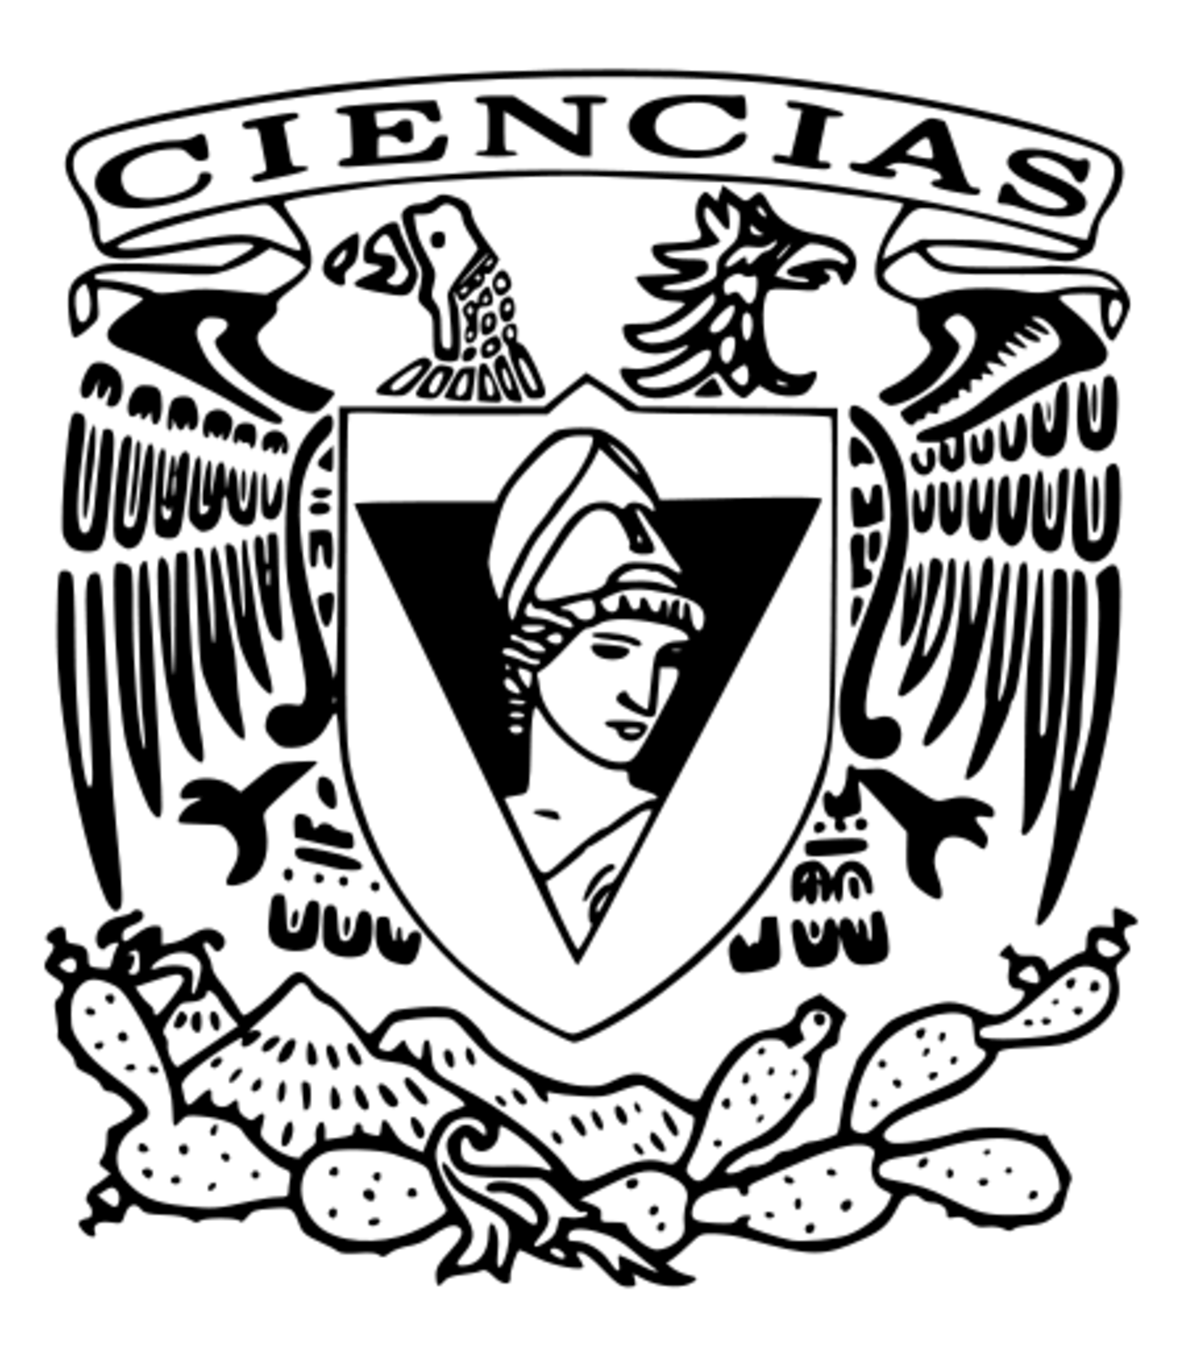
\includegraphics[height=3.2cm]{images/Logo_FC.png}\par}
    \vspace{0.5cm}
    {\scshape\LARGE \textbf{UNIVERSIDAD NACIONAL AUTÓNOMA DE MÉXICO} \par}
    \vspace{0.5cm}
    {\scshape\LARGE FACULTAD DE CIENCIAS \par}
    {\scshape\Large Ciencias de la Computación \par}
    \vspace{0.5cm}
    {\scshape\Huge Compiladores \par}
    {\scshape\Huge Semestre 2027-1 \par}
    \vspace{0.8cm}
    {\scshape\Huge \textbf{Tarea 1} \par}
    {\scshape\Huge \textbf{Introducción y análisis léxico} \par}
    \vspace{0.8cm}
    {\Large Integrantes: \par}
    \vspace{0.5cm}
    \noindent\begin{tabular}{p{10cm}p{3.5cm}}
    \toprule
    \Large
    Escobar Gonzalez Isaac Giovani & \Large 321336400 \\
    \Large
    Garduño Escobar Kevin Jonathan & \Large 321070629 \\
    \Large
    González Gutiérrez Antonio Tonatiuh & \Large 321195476 \\
    \Large
    Zaldivar Alanis Rodrigo & \Large 424029605 \\
    \bottomrule
    \end{tabular}\\
    \vspace{0.8cm}
    {\itshape\Large Fecha de entrega: 13 de Septiembre de 2026 \par}
\end{titlepage}

\begin{enumerate}
    \item Indica los valores asignados a $w, x, y$ y $z$ en los siguientes dos códigos estructurados por bloques.
    Muestra la tabla de símbolos en cada bloque con una implementación imperativa en cada caso:\\
    
    \begin{minipage}{0.5\textwidth}
        \footnotesize
        \begin{verbatim}
    int w, x, y, z;
    int i = 4; int j = 5;
    { 
        int j = 7;
        i = 6;
        w = i + j; 
    } 
    x = i + j;
    {
        int i = 8;
        y = i + j;
    } 
    z = i + j;
        \end{verbatim}
    \end{minipage}
    \begin{minipage}{0.5\textwidth}
        \footnotesize
        \begin{verbatim}
    int w, x, y, z;
    int i = 3; int j = 4;
    {
        int i = 5;
        w = i + j;
    }
    x = i + j;
    {
        int j = 6;
        i = 7;
        y = i + j;
    }
    z = i + j;
        \end{verbatim}
    \end{minipage}

    \noindent\underline{Código izquierdo.}
    \begin{itemize}[nosep]
        \item Global: $i=4,\ j=5$.
        \item Bloque 1: declara $j=7$ local; \texttt{i = 6} es asignación, así que la $i$ global pasa a $6$.
        Entonces $w = i + j = 6 + 7 = 13$. Al salir muere el $j=7$ (vuelve a $5$), pero $i=6$ permanece.
        \item $x = i + j = 6 + 5 = 11$.
        \item Bloque 2: declara $i=8$ local; $y = i + j = 8 + 5 = 13$. Al salir muere el $i=8$ y $i$ vuelve a $6$.
        \item $z = i + j = 6 + 5 = 11$.
    \end{itemize}
    \[ \boxed{w = 13,\quad x = 11,\quad y = 13,\quad z = 11} \]

    Tabla de símbolos por bloque:
    \begin{center}
    \begin{tabular}{ll}
    \toprule
    \textbf{Activo} & \textbf{Contenido de la pila } \\
    \midrule
    Global            & $[\,i{=}4,\ j{=}5,\ w,\ x,\ y,\ z\,]$ \\
    Dentro de Bloque 1 & $[\,i{=}6,\ j{=}5,\dots\,]\ [\,j{=}7\,]$ \\
    Tras salir de B1   & $[\,i{=}6,\ j{=}5,\dots\,]$ \\
    Dentro de Bloque 2 & $[\,i{=}6,\ j{=}5,\dots\,]\ [\,i{=}8\,]$ \\
    Tras salir de B2   & $[\,i{=}6,\ j{=}5,\dots\,]$ \\
    \bottomrule
    \end{tabular}
    \end{center}

    \medskip
    \noindent\underline{Código derecho.}
    \begin{itemize}[nosep]
        \item Global: $i=3,\ j=4$.
        \item Bloque 1: declara $i=5$ local; $w = i + j = 5 + 4 = 9$. Al salir muere el $i=5$ y $i$ vuelve a $3$.
        \item $x = i + j = 3 + 4 = 7$.
        \item Bloque 2: declara $j=6$ local; \texttt{i = 7} es asignación, así que la $i$ global pasa a $7$.
        Entonces $y = i + j = 7 + 6 = 13$. Al salir muere el $j=6$ (vuelve a $4$), pero $i=7$ permanece.
        \item $z = i + j = 7 + 4 = 11$.
    \end{itemize}
    \[ \boxed{w = 9,\quad x = 7,\quad y = 13,\quad z = 11} \]

    Tabla de símbolos por bloque:
    \begin{center}
    \begin{tabular}{ll}
    \toprule
    \textbf{Activo} & \textbf{Contenido de la pila} \\
    \midrule
    Global            & $[\,i{=}3,\ j{=}4,\ w,\ x,\ y,\ z\,]$ \\
    Dentro de Bloque 1 & $[\,i{=}3,\ j{=}4,\dots\,]\ [\,i{=}5\,]$ \\
    Tras salir de B1   & $[\,i{=}3,\ j{=}4,\dots\,]$ \\
    Dentro de Bloque 2 & $[\,i{=}7,\ j{=}4,\dots\,]\ [\,j{=}6\,]$ \\
    Tras salir de B2   & $[\,i{=}7,\ j{=}4,\dots\,]$ \\
    \bottomrule
    \end{tabular}
    \end{center}


    \item Divide el siguiente programa en C++ en lexemas y genera los tokens correspondientes:
    {\footnotesize \begin{verbatim}
        float limitedSquare(x) float x; {
            /* returns x-squared, but never more than 100 */
            return (x<=-10.0||x>=10.0)?100:x*x;
        }
    \end{verbatim}}

    \bigskip
    \noindent\textbf{Solución.} El analizador léxico primero elimina el comentario
        , ya que no produce ningún token. Después separa la entrada en
    lexemas y de ahi cada lexema genera un token de la forma (nombre, atributo); los identificadores
    llevan como atributo un apuntador a la tabla de símbolos.

    \begin{center}
    \begin{tabular}{ll}
    \toprule
    \textbf{Lexema} & \textbf{Token} \\
    \midrule
    \texttt{float}          & \texttt{(keyword, float)} \\
    \texttt{limitedSquare}  & \texttt{(identificador, ->tabla)} \\
    \texttt{(}              & \texttt{(puntuacion, "(")} \\
    \texttt{x}              & \texttt{(identificador, ->tabla)} \\
    \texttt{)}              & \texttt{(puntuacion, ")")} \\
    \texttt{float}          & \texttt{(keyword, float)} \\
    \texttt{x}              & \texttt{(identificador, ->tabla)} \\
    \texttt{;}              & \texttt{(puntuacion, ";")} \\
    \texttt{\{}             & \texttt{(puntuacion, "\{")} \\
    \texttt{return}         & \texttt{(keyword, return)} \\
    \texttt{(}              & \texttt{(puntuacion, "(")} \\
    \texttt{x}              & \texttt{(identificador, ->tabla)} \\
    \texttt{<=}             & \texttt{(operador relacional, LE)} \\
    \texttt{-}              & \texttt{(operador aritmetico, MINUS)} \\
    \texttt{10.0}           & \texttt{(constante, 10.0)} \\
    \texttt{||}             & \texttt{(operador logico, OR)} \\
    \texttt{x}              & \texttt{(identificador, ->tabla)} \\
    \texttt{>=}             & \texttt{(operador relacional, GE)} \\
    \texttt{10.0}           & \texttt{(constante, 10.0)} \\
    \texttt{)}              & \texttt{(puntuacion, ")")} \\
    \texttt{?}              & \texttt{(puntuacion, "?")} \\
    \texttt{100}            & \texttt{(constante, 100)} \\
    \texttt{:}              & \texttt{(puntuacion, ":")} \\
    \texttt{x}              & \texttt{(identificador, ->tabla)} \\
    \texttt{*}              & \texttt{(operador aritmetico, MULT)} \\
    \texttt{x}              & \texttt{(identificador, ->tabla)} \\
    \texttt{;}              & \texttt{(puntuacion, ";")} \\
    \texttt{\}}             & \texttt{(puntuacion, "\}")} \\
    \bottomrule
    \end{tabular}
    \end{center}





    \item Define una función recursiva que compute los prefijos de una una expresión regular. 
    La base de tal función recursiva es:
    \begin{align*}
        prefix(\epsilon) &= \epsilon \\
        prefix(a) &= a?
    \end{align*}
    Completa la definición.

    \bigskip
    \noindent\textbf{Solución.} 

    \begin{align*}
        prefix(\epsilon) &= \epsilon \\
        prefix(a) &= a? \\
        prefix(r \mid s) &= prefix(r) \mid prefix(s) \\
        prefix(r\,s) &= prefix(r) \mid r\cdot prefix(s) \\
        prefix(r^{*}) &= r^{*}\cdot prefix(r)
    \end{align*}

    \noindent Justificación de cada caso:
    \begin{itemize}[nosep]
        \item \textbf{Unión.} Una cadena de $r\mid s$ proviene de $r$ o de $s$, así que sus
        prefijos son los de $r$ o los de $s$.
        \item \textbf{Concatenación.} Un prefijo de $r\,s$ o bien se queda dentro de la
        primera parte (un prefijo de $r$), o bien atraviesa $r$ completo y se detiene dentro
        de la segunda (por eso aparece $r$ entero seguido de un prefijo de $s$). Por ejemplo,
        con $r=ab$ y $s=cd$, los prefijos de $abcd$ son $\{\epsilon, a, ab\}$ (prefijos de
        $r$) junto con $\{abc, abcd\}$ ($r$ completo más un prefijo de $s$).
        \item \textbf{Estrella.} Un prefijo de $r^{*}$ consta de cero o más repeticiones
        completas de $r$ (esto es $r^{*}$) seguidas de un prefijo de una repetición más
        ($prefix(r)$).
    \end{itemize}

    \item Para las siguientes expresiones regulares, da el lenguaje que definen:
    \begin{enumerate}
        \item $[ab][cd\epsilon]$\\
        En este caso, el lenguaje consiste de todas las cadenas de longitud 1 o 2 que comienzan con un símbolo de $\{a,b\}$ y continúan con un símbolo de $\{c,d\}$ o terminan después del primer símbolo, ya que $\epsilon$ esta incluido en el segundo conjunto.
        Por lo tanto, el lenguaje es:
        \[ L = \{ac, ad, a, bc, bd, b\} \]
        \item $[a-zA-Z]^*at^*$\\
        El lenguaje definido por esta expresión regular consiste en todas las cadenas de letras mayúsculas o minúsculas, con la posibilidad de que sea vacía esta primera parte, seguida de la letra 'a' y seguida de cero o más letras 't'. En otras palabras, el lenguaje es:
        \[ L = \{ w \in \{a-z, A-Z\}^* \mid w \text{ termina con 'a' seguido de cero o más 't'} \} \]
        \item $ca[tr]$\\
        Este lenguaje es casí como el primer caso, consiste en todas las cadenas de longitud 3 que comienzan con 'c', seguida de 'a' y terminan con un símbolo de $\{t,r\}$. Por lo tanto, el lenguaje es:
        \[ L = \{cat, car\} \]
    \end{enumerate}
    \item Para el siguiente autómata finito no determinista, construye el autómata finito determinista:
    \begin{center}
        \begin{tikzpicture}[shorten >=1pt, node distance=2cm, on grid, auto, >=Stealth]
            \node[state, initial, initial text=start, accepting] (0) {0};
            \node[state] (1) [right=of 0] {1};
            \node[state] (2) [right=of 1] {2};
            \node[state] (3) [right=of 2] {3};

            \path[->]
            (0) edge node {a} (1)
            (1) edge node {a} (2)
            (2) edge node {a} (3)
            (1) edge [bend left=35] node {b} (0)
            (1) edge [bend right=35] node[swap] {b} (2)
            (3) edge [bend left=35] node {a} (2)
            (3) edge [bend right=35] node[swap] {$\bm{\varepsilon}$} (0);
        \end{tikzpicture}
    \end{center}
    Vamos a seguir el algoritmo de \textbf{Construcción por subconjuntos}:\\
    Primero obtenemos la e-closure del estado inicial y de los estados destino de cada transición que no sea $\varepsilon$:
    \begin{itemize}
        \item e-closure(0) = \{0\}
        \item e-closure(1) = \{1\}
        \item e-closure(2) = \{2\}
        \item e-closure(3) = \{0, 3\}
    \end{itemize}
    Ahora, comenzamos con el estado inicial del DFA, que es e-closure(0) = \{0\}. A partir de este estado, vamos a calcular las transiciones para cada símbolo del alfabeto \{a, b\}:
    \begin{table}[H]
        \centering
        \begin{tabular}{|c|c|c|}
        \hline
        \textbf{Estado} & \textbf{a} & \textbf{b} \\ \hline
        \{0\}           & \{1\}      & $\emptyset$   \\ \hline
        \end{tabular}
    \end{table}
    Como tenemos un estado nuevo \{1\}, calculamos sus transiciones:
    \begin{table}[H]
        \centering
        \begin{tabular}{|c|c|c|}
        \hline
        \textbf{Estado} & \textbf{a} & \textbf{b} \\ \hline
        \{0\}           & \{1\}      & $\emptyset$   \\ \hline
        \{1\}           & \{2\}      & \{0\}      \\ \hline
        \end{tabular}
    \end{table}
    Vemos que tenemos un estado nuevo \{2\}, entonces también calculamos sus transiciones y esto haremos para cada estado nuevo que encontremos hasta que no haya más estados nuevos, por practicidad, omitimos los pasos intermedios y mostramos la tabla final de transiciones del DFA:
    \begin{table}[H]
        \centering
        \begin{tabular}{|c|c|c|}
        \hline
        \textbf{Estado} & \textbf{a}     & \textbf{b} \\ \hline
        \{0\}           & \{1\}          & $\emptyset$   \\ \hline
        \{1\}           & \{2\}          & \{0, 2\}   \\ \hline
        \{2\}           & \{3, 0\}       & $\emptyset$   \\ \hline
        \{0, 2\}        & \{1, 3, 0\}    & $\emptyset$   \\ \hline
        \{3, 0\}        & \{2, 1\}       & $\emptyset$   \\ \hline
        \{1, 3, 0\}     & \{2, 1\}       & \{0, 2\}   \\ \hline
        \{2, 1\}        & \{3, 0, 2\}    & \{0, 2\}   \\ \hline
        \{3, 0, 2\}     & \{2, 1, 3, 0\} & $\emptyset$   \\ \hline
        \{2, 1, 3, 0\}  & \{3, 0, 2, 1\} & \{0, 2\}   \\ \hline
        \end{tabular}
    \end{table}
    De este modo, obtuvimos los estados del DFA y sus transiciones. Los estados de aceptación del DFA son aquellos que contienen al menos un estado de aceptación del NFA original, que en este caso es el estado 0, el estado inicial del DFA será la e-closure del estado inicial del NFA, que es \{0\}. 
    Renombrando los estados del DFA para simplificar y marcando los estados de aceptación e inicial, la tabla final de transiciones del DFA es:
    \begin{table}[H]
        \centering
        \begin{tabular}{|c|c|c|c|c|}
        \hline
        \textbf{Ini/Acept}          & \textbf{Estado} & \textbf{Renombrado} & \textbf{a}     & \textbf{b} \\ \hline
        \textit{Inicial/Aceptación} & \{0\}           & A                   & \{1\} (B)      & $\emptyset$   \\ \hline
        \textit{}                   & \{1\}           & B                   & \{2\} (C)      & \{0, 2\} (D) \\ \hline
        \textit{}                   & \{2\}           & C                   & \{3, 0\} (E)   & $\emptyset$   \\ \hline
        \textit{Aceptación}         & \{0, 2\}        & D                   & \{1, 3, 0\} (F) & $\emptyset$   \\ \hline
        \textit{Aceptación}         & \{3, 0\}        & E                   & \{2, 1\} (G)   & $\emptyset$   \\ \hline
        \textit{Aceptación}         & \{1, 3, 0\}     & F                   & \{2, 1\} (G)   & \{0, 2\} (D) \\ \hline
        \textit{}                   & \{2, 1\}        & G                   & \{3, 0, 2\} (H) & \{0, 2\} (D) \\ \hline
        \textit{Aceptación}         & \{3, 0, 2\}     & H                   & \{2, 1, 3, 0\} (I) & $\emptyset$   \\ \hline
        \textit{Aceptación}         & \{2, 1, 3, 0\}  & I                   & \{3, 0, 2, 1\} (I) & \{0, 2\} (D) \\ \hline
        \end{tabular}
    \end{table}
    Ahora podemos dibujar el DFA resultante:
    \begin{center}
        \begin{tikzpicture}[shorten >=1pt, node distance=2cm, on grid, auto, >=Stealth]
            
            % Fila superior
            \node[state, initial, initial text=start, accepting] (A) {A};
            \node[state] (B) [right=of A] {B};
            \node[state] (C) [right=of B] {C};
            \node[state, accepting] (E) [right=of C] {E};

            % Fila inferior
            \node[state, accepting] (D) [below=of B] {D};
            \node[state, accepting] (F) [right=of D] {F};
            \node[state] (G) [right=of F] {G};
            \node[state, accepting] (H) [right=of G] {H};
            \node[state, accepting] (I) [right=of H] {I};

            \path[->]
            % Transiciones horizontales (Fila superior)
            (A) edge node {$a$} (B)
            (B) edge node {$a$} (C)
            (C) edge node {$a$} (E)
            
            % Transiciones verticales hacia la fila inferior
            (B) edge node[swap] {$b$} (D)
            (E) edge node {$a$} (G)

            % Transiciones horizontales hacia la derecha (Fila inferior)
            (D) edge node {$a$} (F)
            (F) edge node {$a$} (G)
            (G) edge node {$a$} (H)
            (H) edge node {$a$} (I)
            
            % Ciclo sobre sí mismo en el estado I
            (I) edge [out=90, in=0, loop] node {$a$} (I)

            % Transiciones de regreso con 'b' hacia el estado D
            (F) edge [bend left=40] node[below] {$b$} (D)
            (G) edge [bend left=50] node[below] {$b$} (D)
            (I) edge [bend left=60] node[below] {$b$} (D);
        \end{tikzpicture}
    \end{center}
    \item Para los siguientes DFA obten el DFA mínimo:
    \begin{enumerate}
        \item 
        \begin{tikzpicture}[shorten >=1pt, auto, >=Stealth]
            \node[state, initial above, initial text=, accepting] (0) at (0,0) {0};
            \node[state] (1) at (2.5, -1.5) {1};
            \node[state] (2) at (1.5, -4) {2};
            \node[state] (3) at (-1.5, -4) {3};
            \node[state] (4) at (-2.5, -1.5) {4};

            \path[->]
            (0) edge node {a} (1)
            (0) edge node[swap] {b} (2)
            (1) edge node {a} (2)
            (2) edge node {a} (3)
            (3) edge node {b} (0)
            (4) edge node {b} (0)
            
            (3) edge [bend left] node {a} (4)
            (4) edge [bend left] node {a} (3);
        \end{tikzpicture}

        Primero vamos a dividir en grupos de estados finales y no finales:
        \begin{align*}
            G_1 &= \{0\} \\
            G_2 &= \{1, 2, 3, 4\}
        \end{align*}
        Luego, tomamos a $G_1$ y por definición de grupo consistente tenemos que $G_1$ es consistente, ya que es un grupo de un solo estado, entonces marcamos $G_1$ y quedan los grupos:
        \begin{align*}
            \ast G_1 &= \{0\} \\
            G_2 &= \{1, 2, 3, 4\}
        \end{align*}
        Ahora, tomamos a $G_2$ y hacemos su tabla de estados:
        \begin{table}[H]
            \centering
            \begin{tabular}{|c|c|c|}
            \hline
            $\bm{G_2}$ & \textbf{a} & \textbf{b} \\ \hline
            1             & $G_2$       & -          \\ \hline
            2             & $G_2$       & -          \\ \hline
            3             & $G_2$       & $G_1$       \\ \hline
            4             & $G_2$       & $G_1$       \\ \hline
            \end{tabular}
        \end{table}
        $G_2$ no es consistente ya que no todas sus filas son iguales, entonces dividimos $G_2$ en dos grupos de manera que sus filas sean iguales, desmarcamos grupos y borramos a $G_2$ y nos quedan los grupos:
        \begin{align*}
            G_1 &= \{0\} \\
            G_3 &= \{1, 2\} \\
            G_4 &= \{3, 4\}
        \end{align*}
        Y volvemos a hacer lo mismo, tomamos a $G_1$ y como es un grupo de un solo estado, es consistente, entonces marcamos $G_1$ y nos quedan los grupos:
        \begin{align*}
            \ast G_1 &= \{0\} \\
            G_3 &= \{1, 2\} \\
            G_4 &= \{3, 4\}
        \end{align*}
        Ahora, tomamos a $G_3$ y hacemos su tabla de estados:
        \begin{table}[H]
            \centering
            \begin{tabular}{|c|c|c|}
            \hline
            $\bm{G_3}$ & \textbf{a} & \textbf{b} \\ \hline
            1             & $G_3$       & -          \\ \hline
            2             & $G_4$       & -          \\ \hline
            \end{tabular}
        \end{table}
        $G_3$ no es consistente ya que no todas sus filas son iguales, entonces dividimos $G_3$ en grupos de las filas iguales, desmarcamos grupos y borramos a $G_3$ y nos quedan los grupos:
        \begin{align*}
            G_1 &= \{0\} \\
            G_4 &= \{3, 4\} \\
            G_5 &= \{1\} \\
            G_6 &= \{2\} 
        \end{align*}
        Dado que $G_1, G_5$ y $G_6$ son grupos de un solo estado, son consistentes, entonces marcamos $G_1, G_5$ y $G_6$ y nos quedan los grupos:
        \begin{align*}
            \ast G_1 &= \{0\} \\
            G_4 &= \{3, 4\} \\
            \ast G_5 &= \{1\} \\
            \ast G_6 &= \{2\}
        \end{align*}
        Tomamos a $G_4$ y hacemos su tabla de estados:
        \begin{table}[H]
            \centering
            \begin{tabular}{|c|c|c|}
            \hline
            $\bm{G_4}$ & \textbf{a} & \textbf{b} \\ \hline
            3             & $G_4$       & $G_1$       \\ \hline
            4             & $G_4$       & $G_1$       \\ \hline
            \end{tabular}
        \end{table}
        Vemos que $G_4$ es consistente, ya que todas sus filas son iguales, entonces marcamos $G_4$ y nos quedan los grupos:
        \begin{align*}
            \ast G_1 &= \{0\} \\
            \ast G_4 &= \{3, 4\} \\
            \ast G_5 &= \{1\} \\
            \ast G_6 &= \{2\}
        \end{align*}
        Todos los grupos están marcados, entonces ahora si cada grupo va a ser un estado del nuevo DFA y para las transiciones por el algoritmo tenemos que si un estado $p$ en el DFA original va a un estado $q$ por el símbolo $a$, entonces el grupo que contiene a $p$ va a ir al grupo que contiene a $q$ por el símbolo $a$.\\
        Además, el estado inicial del nuevo DFA va a ser el grupo que contiene al estado inicial del DFA original y los estados de aceptación del nuevo DFA van a ser los grupos que contienen a los estados de aceptación del DFA original.\\
        Por lo tanto, el DFA mínimo es:
        \begin{center}
            \begin{tikzpicture}[shorten >=1pt, node distance=3cm, auto, >=Stealth]
            
                \node[state, initial, initial text=start, accepting] (G1) {$G_1$};
                \node[state] (G5) [right=of G1] {$G_5$};
                \node[state] (G4) [below=of G1] {$G_4$};
                \node[state] (G6) [below=of G5] {$G_6$};

                \path[->]
                (G1) edge node {$a$} (G5)
                (G5) edge node {$a$} (G6)
                (G6) edge node {$a$} (G4)
                (G4) edge node {$b$} (G1)
                
                (G1) edge node [pos=0.3] {$b$} (G6)
                
                (G4) edge [out=270, in=180, loop] node {$a$} (G4);
            \end{tikzpicture}
        \end{center}
        \item 
        \begin{tikzpicture}[shorten >=1pt, auto, >=Stealth, node distance=2cm]
            \node[state, initial, initial text=] (0) {0};
            \node[state] (1) [right=of 0] {1};
            \node[state] (2) [right=of 1] {2};
            
            \node[state] (3) [below=of 0] {3};
            \node[state, accepting] (4) [below=of 1] {4};
            \node[state] (5) [below=of 2] {5};

            \path[->]
            (0) edge node {b} (1)
            (0) edge node[swap] {a} (3)
            (1) edge node {a} (2)
            (3) edge node {b} (4)
            (4) edge node {b} (5)
            
            (1) edge [bend right] node[swap] {b} (4)
            (4) edge [bend right] node[swap] {a} (1)
            
            (2) edge [bend right] node[swap] {b} (5)
            (5) edge [bend right] node[swap] {b} (2)
            
            (2) edge [out=90, in=0, loop] node {a} (2)
            (5) edge [out=270, in=0, loop] node {a} (5);
        \end{tikzpicture}

        % Estructura: \fcolorbox{ColorDelBorde}{ColorDelFondo}{Tu Texto}
        \fcolorbox{red}{yellow!10}{\textbf{Nota importante:} Esta bajo revisión, tengo dudas así que no se si esta bien.}

        Dividimos en grupos de estados finales y no finales:
        \begin{align*}
            G_1 &= \{4\} \\
            G_2 &= \{0, 1, 2, 3, 5\}
        \end{align*}
        Tomamos a $G_1$ y como es un grupo de un solo estado, es consistente, entonces marcamos $G_1$ y nos quedan los grupos:
        \begin{align*}
            \ast G_1 &= \{4\} \\
            G_2 &= \{0, 1, 2, 3, 5\}
        \end{align*}
        Ahora, tomamos a $G_2$ y hacemos su tabla de estados:
        \begin{table}[H]
            \centering
            \begin{tabular}{|c|c|c|}
            \hline
            $\bm{G_2}$ & \textbf{a} & \textbf{b} \\ \hline
            0             & $G_2$       & $G_2$       \\ \hline
            1             & $G_2$       & $G_1$       \\ \hline
            2             & $G_2$       & $G_2$       \\ \hline
            3             & -           & $G_1$       \\ \hline
            5             & $G_2$       & $G_2$       \\ \hline
            \end{tabular}
        \end{table}
        $G_2$ no tiene todas sus filas iguales por lo que no es consistente, entonces dividimos $G_2$ en grupos con las filas iguales, desmarcamos grupos y borramos a $G_2$ y nos quedan los grupos:
        \begin{align*}
            G_1 &= \{4\} \\
            G_3 &= \{0, 2, 5\} \\
            G_4 &= \{1\} \\
            G_5 &= \{3\}
        \end{align*}
        Dado que $G_1, G_4$ y $G_5$ son grupos de un solo estado, entonces son consistentes, así que marcamos $G_1, G_4$ y $G_5$ y nos quedan los grupos:
        \begin{align*}
            \ast G_1 &= \{4\} \\
            G_3 &= \{0, 2, 5\} \\
            \ast G_4 &= \{1\} \\
            \ast G_5 &= \{3\}
        \end{align*}
        Ahora, tomamos a $G_3$ y hacemos su tabla de estados:
        \begin{table}[H]
            \centering
            \begin{tabular}{|c|c|c|}
            \hline
            $\bm{G_3}$ & \textbf{a} & \textbf{b} \\ \hline
            0             & $G_5$   & $G_4$       \\ \hline
            2             & $G_3$   & $G_3$       \\ \hline
            5             & $G_3$   & $G_3$       \\ \hline
            \end{tabular}
        \end{table}
        $G_3$ no es consistente, entonces dividimos $G_3$ en grupos de filas iguales, desmarcamos grupos y borramos a $G_3$ y nos quedan los grupos:
        \begin{align*}
            G_1 &= \{4\} \\
            G_4 &= \{1\} \\
            G_5 &= \{3\} \\
            G_6 &= \{0\} \\
            G_7 &= \{2, 5\}
        \end{align*}
        $G_1, G_4, G_5$ y $G_6$ son grupos de un solo estado, entonces son consistentes, los marcamos y nos quedan los grupos:
        \begin{align*}
            \ast G_1 &= \{4\} \\
            \ast G_4 &= \{1\} \\
            \ast G_5 &= \{3\} \\
            \ast G_6 &= \{0\} \\
            G_7 &= \{2, 5\}
        \end{align*}
        Luego, tomamos a $G_7$ y hacemos su tabla de estados: 
        \begin{table}[H]
            \centering
            \begin{tabular}{|c|c|c|}
            \hline
            $\bm{G_7}$ & \textbf{a} & \textbf{b} \\ \hline
            2             & $G_7$   & $G_7$       \\ \hline
            5             & $G_7$   & $G_7$       \\ \hline
            \end{tabular}
        \end{table}
        Así $G_7$ es consistente, entonces lo marcamos y nos quedan los grupos:
        \begin{align*}
            \ast G_1 &= \{4\} \\
            \ast G_4 &= \{1\} \\
            \ast G_5 &= \{3\} \\
            \ast G_6 &= \{0\} \\
            \ast G_7 &= \{2, 5\}
        \end{align*}
        Todos los grupos están marcados, entonces ahora si cada grupo va a ser un estado del nuevo DFA y hacemos lo mismo que en el ejercicio anterior para las transiciones, estado inicial y estados de aceptación.\\
        Por lo tanto, el DFA mínimo es:
        \begin{center}
            \begin{tikzpicture}[shorten >=1pt, node distance=2cm, auto, >=Stealth]
                
                % Definición de estados y distribución espacial
                \node[state, initial, initial text=start] (G6) {$G_6$};
                \node[state] (G4) [right=of G6] {$G_4$};
                \node[state, accepting] (G1) [right=of G4] {$G_1$};
                \node[state] (G5) [above=of G4] {$G_5$};
                
                % G7 se desplaza en X para quedar exactamente centrado debajo de G4 y G1
                \node[state] (G7) [below=of G4, xshift=1.5cm] {$G_7$};

                \path[->]
                % Transiciones desde el estado inicial G6
                (G6) edge node {$a$} (G5)
                (G6) edge node {$b$} (G4)
                
                % Transición superior desde G5
                (G5) edge node {$b$} (G1)
                
                % Transiciones mutuas entre G4 y G1
                (G4) edge [bend left] node {$b$} (G1)
                (G1) edge [bend left] node {$a$} (G4)
                
                % Transiciones hacia el estado sumidero G7
                (G4) edge node[swap] {$a$} (G7)
                (G1) edge node {$b$} (G7)
                
                % Ciclos sobre G7 agrupados en una sola flecha
                (G7) edge [loop below] node {$a, b$} (G7);
            \end{tikzpicture}
        \end{center}
    \end{enumerate}
    \item Convierte las siguientes expresiones regulares en autómatas finitos deterministas (DFA):
    \begin{enumerate}
        \item $[ab]^*$
        \item $(a?b^*)^*$
        \item $[ab]^*abb[ab]^*$
    \end{enumerate}

    \textbf{Respuesta:}

    Para cada expresión regular, primero preprocesamos la expresión haciendo
    explícitas las concatenaciones (representadas con $\cdot$). Después
    aplicamos el algoritmo de \textbf{Shunting Yard} para convertirla a notación
    postfija. A partir de la expresión postfija aplicamos el algoritmo de
    construcción de \textbf{Thompson} para obtener un $\varepsilon$-NFA.
    Finalmente, aplicamos el algoritmo de determinización
    $\text{NFA}\rightarrow\text{DFA}$ mediante la \textbf{construcción de subconjuntos}.

    En la construcción del DFA, cada nuevo estado (denotado con letras mayúsculas) 
    representa un conjunto de estados del $\varepsilon$-NFA. Para cada conjunto $S$ y 
    cada símbolo $a\in\Sigma$, calculamos las transiciones como:
    \[
        \delta_D(S,a)=EC(move(S,a)),
    \]
    donde $EC$ representa la cerradura-$\varepsilon$. 
    También, recordemos que un estado del DFA es de aceptación si el subconjunto contiene al menos un estado de 
    aceptación del NFA original.

    Las precedencias (para el algoritmo de Shunting Yard) son:
    clausuras ($*$, $?$) $>$ concatenación ($\cdot$) $>$ unión ($|$).

    \begin{enumerate}

        % Inciso A

        \item $[ab]^*$ equivale a $(a|b)^*$

        \textbf{Algoritmo de Shunting Yard}

        \begin{center}
            \small
            \begin{tabular}{lll}
                \toprule
                \textbf{Token/Símbolo} & \textbf{Pila de operadores} & \textbf{Salida (Postfija)} \\
                \midrule
                \texttt{(} & \texttt{(} & \\
                \texttt{a} & \texttt{(} & \texttt{a} \\
                \texttt{|} & \texttt{( |} & \texttt{a} \\
                \texttt{b} & \texttt{( |} & \texttt{a b} \\
                \texttt{)} & Vacía & \texttt{a b |} \\
                \texttt{*} & \texttt{*} & \texttt{a b |} \\
                Fin de cadena & Vacía & \texttt{a b | *} \\
                \bottomrule
            \end{tabular}
        \end{center}

        Expresión postfija: $\boxed{\texttt{a b | *}}$

        \textbf{Construcción de Thompson (NFA)}

        Para construir el autómata a partir de la expresión postfija \texttt{a b | *}, evaluamos los operadores de izquierda a derecha. Primero, el operador de unión \texttt{|} toma los subautómatas de \texttt{a} y \texttt{b}, creando una bifurcación con transiciones $\varepsilon$ para elegir cualquiera de los dos caminos. Luego, el operador de cerradura de Kleene \texttt{*} toma todo el bloque anterior y le agrega un nuevo estado inicial y uno final, incorporando transiciones $\varepsilon$ que permiten hacer un ciclo continuo (repetición) o saltar directamente al final (aceptar la cadena vacía).

        \begin{center}
            \begin{tikzpicture}[shorten >=1pt, node distance=1.5cm, auto, >=Stealth]
                \node[state, initial, initial text=start] (0) {0};
                \node[state] (1) [right=of 0] {1};
                \node[state] (2) [above right=0.5cm and 1cm of 1] {2};
                \node[state] (3) [right=of 2] {3};
                \node[state] (4) [below right=0.5cm and 1cm of 1] {4};
                \node[state] (5) [right=of 4] {5};
                \node[state] (6) [below right=0.5cm and 1cm of 3] {6};
                \node[state, accepting] (7) [right=of 6] {7};

                \path[->]
                (0) edge node {$\varepsilon$} (1)
                (1) edge node {$\varepsilon$} (2)
                (1) edge node[swap] {$\varepsilon$} (4)
                (2) edge node {$a$} (3)
                (4) edge node[swap] {$b$} (5)
                (3) edge node {$\varepsilon$} (6)
                (5) edge node[swap] {$\varepsilon$} (6)
                (6) edge node {$\varepsilon$} (7)
                (6) edge [bend right=90] node[above] {$\varepsilon$} (1)
                (0) edge [bend right=60] node[above] {$\varepsilon$} (7);
            \end{tikzpicture}
        \end{center}

        \textbf{Determinización a DFA mediante construcción de subconjuntos}

        Definimos los estados del DFA calculando las cerraduras-$\varepsilon$ iterativamente. El estado de aceptación del NFA es $7$:
        \begin{align*}
            A &= EC(\{0\}) = \{0,1,2,4,7\} \quad \text{(Aceptación)}\\
            B &= EC(move(A, a)) = \{1,2,3,4,6,7\} \quad \text{(Aceptación)}\\
            C &= EC(move(A, b)) = \{1,2,4,5,6,7\} \quad \text{(Aceptación)}
        \end{align*}

        Resumiendo los cálculos en su tabla de transiciones:
        \begin{center}
            \small
            \begin{tabular}{c|cc}
                \toprule
                \textbf{Estado DFA} & \textbf{Con $a$} & \textbf{Con $b$} \\
                \midrule
                $\rightarrow *A$ & $B$ & $C$ \\
                $*B$ & $B$ & $C$ \\
                $*C$ & $B$ & $C$ \\
                \bottomrule
            \end{tabular}
        \end{center}

        El DFA obtenido es:

        \begin{center}
            \begin{tikzpicture}[shorten >=1pt, node distance=2.5cm, auto, >=Stealth]
                \node[state, initial, initial text=start, accepting] (A) {$A$};
                \node[state, accepting] (B) [right=of A] {$B$};
                \node[state, accepting] (C) [below=of B] {$C$};

                \path[->]
                (A) edge node {$a$} (B)
                (A) edge node[swap] {$b$} (C)
                (B) edge [loop above] node {$a$} (B)
                (B) edge [bend left=15] node {$b$} (C)
                (C) edge [bend left=15] node {$a$} (B)
                (C) edge [loop below] node {$b$} (C);
            \end{tikzpicture}
        \end{center}

        % Inciso B

        \item $(a?b^*)^*$ equivale a $((a|\varepsilon)\cdot b^*)^*$

        \textbf{Algoritmo de Shunting Yard}

        \begin{center}
            \small
            \begin{tabular}{lll}
                \toprule
                \textbf{Token/Símbolo} & \textbf{Pila de operadores} & \textbf{Salida (Postfija)} \\
                \midrule
                \texttt{(} & \texttt{(} & \\
                \texttt{a} & \texttt{(} & \texttt{a} \\
                \texttt{?} & \texttt{(} & \texttt{a ?} \\
                \texttt{$\cdot$} & \texttt{( $\cdot$} & \texttt{a ?} \\
                \texttt{b} & \texttt{( $\cdot$} & \texttt{a ? b} \\
                \texttt{*} & \texttt{( $\cdot$ *} & \texttt{a ? b} \\
                \texttt{)} & Vacía & \texttt{a ? b * $\cdot$} \\
                \texttt{*} & \texttt{*} & \texttt{a ? b * $\cdot$} \\
                Fin de cadena & Vacía & \texttt{a ? b * $\cdot$ *} \\
                \bottomrule
            \end{tabular}
        \end{center}

        Expresión postfija: $\boxed{\texttt{a ? b * $\cdot$ *}}$

        \textbf{Construcción de Thompson (NFA)}

        Siguiendo la expresión postfija, primero se construye el bloque \texttt{a ?} (que es equivalente a $a|\varepsilon$), creando un camino para leer $a$ y otro para saltarlo mediante una transición $\varepsilon$. Posteriormente, se construye el ciclo para \texttt{b *} usando la estructura estándar de Kleene. El operador de concatenación $\cdot$ une el estado final del bloque \texttt{a ?} con el inicial de \texttt{b *} mediante una única transición $\varepsilon$. Finalmente, el operador de cerradura \texttt{*} exterior envuelve toda esta secuencia concatenada, agregando transiciones $\varepsilon$ globales para repetir todo el patrón o evadirlo por completo.

        \begin{center}
            \hspace*{-1cm} % Desplaza el autómata a la izquierda
            \resizebox{0.95\textwidth}{!}{
            \begin{tikzpicture}[shorten >=1pt, node distance=1.2cm, auto, >=Stealth]
                \node[state, initial, initial text=start] (0) {0};
                \node[state] (1) [right=of 0] {1};
                \node[state] (2) [above right=0.5cm and 1cm of 1] {2};
                \node[state] (3) [right=of 2] {3};
                \node[state] (4) [below right=0.5cm and 1cm of 1] {4};
                \node[state] (5) [right=of 4] {5};
                \node[state] (6) [below right=0.5cm and 1cm of 3] {6};
                \node[state] (7) [right=of 6] {7};
                \node[state] (8) [right=of 7] {8};
                \node[state] (9) [right=of 8] {9};
                \node[state] (10) [right=of 9] {10};
                \node[state] (11) [right=of 10] {11};
                \node[state, accepting] (12) [right=of 11] {12};

                \path[->]
                (0) edge node {$\varepsilon$} (1)
                (1) edge node {$\varepsilon$} (2)
                (1) edge node[swap] {$\varepsilon$} (4)
                (2) edge node {$a$} (3)
                (4) edge node[swap] {$\varepsilon$} (5)
                (3) edge node {$\varepsilon$} (6)
                (5) edge node[swap] {$\varepsilon$} (6)
                (6) edge node {$\varepsilon$} (7)
                (7) edge node {$\varepsilon$} (8)
                (8) edge node {$b$} (9)
                (9) edge node {$\varepsilon$} (10)
                (9) edge [bend right=45] node[above] {$\varepsilon$} (8)
                (7) edge [bend right=45] node[swap] {$\varepsilon$} (10)
                (10) edge node {$\varepsilon$} (11)
                (11) edge node {$\varepsilon$} (12)
                (11) edge [bend right=60] node[above] {$\varepsilon$} (1)
                (0) edge [bend right=45] node[swap] {$\varepsilon$} (12);
            \end{tikzpicture}
            }
        \end{center}

        \textbf{Determinización a DFA mediante construcción de subconjuntos}

        Definimos los estados del DFA calculando las cerraduras-$\varepsilon$ iterativamente. El estado de aceptación del NFA es $12$:
        \begin{align*}
            A &= EC(\{0\}) = \{0,1,2,4,5,6,7,8,10,11,12\} \quad \text{(Aceptación)}\\
            B &= EC(move(A, a)) = \{1,2,3,4,5,6,7,8,10,11,12\} \quad \text{(Aceptación)}\\
            C &= EC(move(A, b)) = \{1,2,4,5,6,7,8,9,10,11,12\} \quad \text{(Aceptación)}
        \end{align*}

        Resumiendo los cálculos en su tabla de transiciones:
        \begin{center}
            \small
            \begin{tabular}{c|cc}
                \toprule
                \textbf{Estado DFA} & \textbf{Con $a$} & \textbf{Con $b$} \\
                \midrule
                $\rightarrow *A$ & $B$ & $C$ \\
                $*B$ & $B$ & $C$ \\
                $*C$ & $B$ & $C$ \\
                \bottomrule
            \end{tabular}
        \end{center}

        El DFA obtenido mediante la construcción de subconjuntos es:

        \begin{center}
            \begin{tikzpicture}[shorten >=1pt, node distance=2.5cm, auto, >=Stealth]
                \node[state, initial, initial text=start, accepting] (A) {$A$};
                \node[state, accepting] (B) [right=of A] {$B$};
                \node[state, accepting] (C) [below=of B] {$C$};

                \path[->]
                (A) edge node {$a$} (B)
                (A) edge node[swap] {$b$} (C)
                (B) edge [loop above] node {$a$} (B)
                (B) edge [bend left=15] node {$b$} (C)
                (C) edge [bend left=15] node {$a$} (B)
                (C) edge [loop below] node {$b$} (C);
            \end{tikzpicture}
        \end{center}

        % Inciso C

        \item $[ab]^*abb[ab]^*$ equivale a $(a|b)^*\cdot a\cdot b\cdot b\cdot(a|b)^*$

        \textbf{Algoritmo de Shunting Yard}

        La expresión con las concatenaciones explícitas es: $(a|b)^*\cdot a\cdot b\cdot b\cdot(a|b)^*$ \\
        Su expresión postfija es:
        $\boxed{\texttt{a b | * a $\cdot$ b $\cdot$ b $\cdot$ a b | * $\cdot$}}$

        \textbf{Construcción de Thompson (NFA)}

        Al leer la postfija, ensamblamos el autómata conectando bloques secuencialmente. Ya construimos el bloque \texttt{a b | *} en el inciso A (una unión dentro de una cerradura de Kleene), por lo que lo instanciamos una vez al inicio y otra al final. En la parte intermedia, se crean simples transiciones directas para leer la secuencia exacta \texttt{a}, \texttt{b}, \texttt{b}. Cada vez que aparece el operador de concatenación $\cdot$ en la postfija, este se encarga de enlazar el estado de aceptación del bloque recién terminado con el estado inicial del bloque siguiente mediante una sola transición $\varepsilon$. Así, se forma una cadena principal que conecta todas las partes.

        \begin{center}
            \hspace*{-1cm} % Desplaza el autómata a la izquierda
            \resizebox{0.95\textwidth}{!}{
            \begin{tikzpicture}[shorten >=1pt, node distance=1.2cm, auto, >=Stealth]
                \node[state, initial, initial text=start] (0) {0};
                \node[state] (1) [right=of 0] {1};
                \node[state] (2) [above right=0.4cm and 0.8cm of 1] {2};
                \node[state] (3) [right=of 2] {3};
                \node[state] (4) [below right=0.4cm and 0.8cm of 1] {4};
                \node[state] (5) [right=of 4] {5};
                \node[state] (6) [below right=0.4cm and 0.8cm of 3] {6};
                \node[state] (7) [right=of 6] {7};
                \node[state] (8) [right=of 7] {8};
                \node[state] (9) [right=of 8] {9};
                \node[state] (10) [right=of 9] {10};
                \node[state] (11) [right=of 10] {11};
                \node[state] (12) [right=of 11] {12};
                \node[state] (13) [above right=0.4cm and 0.8cm of 12] {13};
                \node[state] (14) [right=of 13] {14};
                \node[state] (15) [below right=0.4cm and 0.8cm of 12] {15};
                \node[state] (16) [right=of 15] {16};
                \node[state] (17) [below right=0.4cm and 0.8cm of 14] {17};
                \node[state, accepting] (18) [right=of 17] {18};

                \path[->]
                (0) edge node {$\varepsilon$} (1)
                (1) edge node {$\varepsilon$} (2)
                (1) edge node[swap] {$\varepsilon$} (4)
                (2) edge node {$a$} (3)
                (4) edge node[swap] {$b$} (5)
                (3) edge node {$\varepsilon$} (6)
                (5) edge node[swap] {$\varepsilon$} (6)
                (6) edge node {$\varepsilon$} (7)
                (6) edge [bend right=100] node[above] {$\varepsilon$} (1)
                (0) edge [bend right=70] node[swap] {$\varepsilon$} (7)
                (7) edge node {$a$} (8)
                (8) edge node {$b$} (9)
                (9) edge node {$b$} (10)
                (10) edge node {$\varepsilon$} (11)
                (11) edge node {$\varepsilon$} (12)
                (12) edge node {$\varepsilon$} (13)
                (12) edge node[swap] {$\varepsilon$} (15)
                (13) edge node {$a$} (14)
                (15) edge node[swap] {$b$} (16)
                (14) edge node {$\varepsilon$} (17)
                (16) edge node[swap] {$\varepsilon$} (17)
                (17) edge node {$\varepsilon$} (18)
                (17) edge [bend right=100] node[above] {$\varepsilon$} (12)
                (11) edge [bend right=70] node[swap] {$\varepsilon$} (18);
            \end{tikzpicture}
            }
        \end{center}

        \textbf{Determinización a DFA mediante construcción de subconjuntos}

        Definimos los estados del DFA calculando las cerraduras-$\varepsilon$ iterativamente. El estado de aceptación del NFA es $18$:
        \begin{align*}
            A &= EC(\{0\}) = \{0,1,2,4,7\} \\
            B &= EC(move(A, a)) = \{1,2,3,4,6,7,8\} \\
            C &= EC(move(A, b)) = \{1,2,4,5,6,7\} \\
            D &= EC(move(B, b)) = \{1,2,4,5,6,7,9\} \\
            E &= EC(move(D, b)) = \{1,2,4,5,6,7,10,11,12,13,15,18\} \quad \text{(Aceptación)}\\
            F &= EC(move(E, a)) = \{1,2,3,4,6,7,8,12,13,14,15,17,18\} \quad \text{(Aceptación)}\\
            G &= EC(move(E, b)) = \{1,2,4,5,6,7,12,13,15,16,17,18\} \quad \text{(Aceptación)}\\
            H &= EC(move(F, b)) = \{1,2,4,5,6,7,9,12,13,15,16,17,18\} \quad \text{(Aceptación)}\\
            I &= EC(move(H, b)) = \{1,2,4,5,6,7,10,11,12,13,15,16,17,18\} \quad \text{(Aceptación)}
        \end{align*}

        Resumiendo los cálculos en su tabla de transiciones:
        \begin{center}
            \begin{tabular}{c|cc}
                \toprule
                \textbf{Estado DFA} & \textbf{Con $a$} & \textbf{Con $b$} \\
                \midrule
                $\rightarrow A$ & $B$ & $C$ \\
                $B$ & $B$ & $D$ \\
                $C$ & $B$ & $C$ \\
                $D$ & $B$ & $E$ \\
                $*E$ & $F$ & $G$ \\
                $*F$ & $F$ & $H$ \\
                $*G$ & $F$ & $G$ \\
                $*H$ & $F$ & $I$ \\
                $*I$ & $F$ & $G$ \\
                \bottomrule
            \end{tabular}
        \end{center}

        Por lo tanto, el DFA obtenido directamente mediante el algoritmo
        de determinización es:

        \begin{center}
            \hspace*{-1.5cm}
            \begin{tikzpicture}[
                shorten >=1pt,
                node distance=1.7cm,
                auto,
                >=Stealth
            ]
                \node[state, initial, initial text=start] (A) {$A$};
                \node[state] (B) [right=of A] {$B$};
                \node[state] (C) [below=of A] {$C$};
                \node[state] (D) [right=of C] {$D$};
                \node[state, accepting] (E) [right=of D] {$E$};

                \node[state, accepting] (F) [above right=of E] {$F$};
                \node[state, accepting] (G) [below right=of E] {$G$};
                \node[state, accepting] (H) [right=of G] {$H$};
                \node[state, accepting] (I) [above right=of H] {$I$};

                \path[->]
                (A) edge node {$a$} (B)
                (A) edge node[swap] {$b$} (C)

                (B) edge [loop above] node {$a$} (B)
                (B) edge [bend left=15] node {$b$} (D) 

                (C) edge node {$a$} (B)
                (C) edge [loop below] node {$b$} (C)

                (D) edge [bend left=15] node {$a$} (B)
                (D) edge node {$b$} (E)

                (E) edge node {$a$} (F)
                (E) edge node[swap] {$b$} (G)

                (F) edge [loop above] node {$a$} (F)
                (F) edge [bend left=15] node {$b$} (H)

                (G) edge node {$a$} (F)
                (G) edge [loop below] node {$b$} (G)

                (H) edge [bend left=15] node {$a$} (F)
                (H) edge node {$b$} (I)

                (I) edge [bend right=20] node[swap] {$a$} (F)
                (I) edge [bend left=60] node {$b$} (G);
            \end{tikzpicture}
        \end{center}

    \end{enumerate}


    \item Utiliza el algoritmo de simulación de NFA para simular los siguientes NFAs en la entrada $aabb$:
    \begin{enumerate}
        \item 
        \begin{tikzpicture}[shorten >=1pt, node distance=2cm, auto, >=Stealth]
            \node[state, initial, initial text=start] (0) {0};
            \node[state] (1) [right=of 0] {1};
            \node[state] (2) [right=of 1] {2};
            \node[state, accepting] (3) [right=of 2] {3};

            \path[->]
            (0) edge node {$\bm{a}$} (1)
            (1) edge node {$\bm{a}$} (2)
            (2) edge node {$\bm{b}$} (3)
            
            (0) edge [out=335, in=205, loop] node {$\bm{a, b}$} (0)
            (1) edge [out=335, in=205, loop] node {$\bm{a, b}$} (1)
            (2) edge [out=335, in=205, loop] node {$\bm{a, b}$} (2)
            
            (2) edge [bend right=45] node[above] {$\bm{\varepsilon}$} (0);
        \end{tikzpicture}

        \textbf{Respuesta:}
        
        Primero obtenemos las cerraduras epsilon ($\varepsilon$-closures o $EC$) para cada estado:
        
        \[ EC(0) = \{0\}, \quad EC(1) = \{1\}, \quad EC(2) = \{0, 2\}, \quad EC(3) = \{3\} \]
        
        Evaluamos la cadena $aabb\$$ paso a paso:
        \begin{itemize}
            \item Estado inicial: $S = EC(0) = \{0\}$. Leemos $c = a$.
            \[ S = EC(\delta(\{0\}, a)) = EC(\{0, 1\}) = EC(0) \cup EC(1) = \{0, 1\} \]
            \item Estado actual: $S = \{0, 1\}$. Leemos $c = a$.
            \[ S = EC(\delta(\{0, 1\}, a)) = EC(\{0, 1, 2\}) = EC(0) \cup EC(1) \cup EC(2) = \{0, 1, 2\} \]
            \item Estado actual: $S = \{0, 1, 2\}$. Leemos $c = b$.
            \[ S = EC(\delta(\{0, 1, 2\}, b)) = EC(\{0, 1, 2, 3\}) = \{0, 1, 2, 3\} \]
            \item Estado actual: $S = \{0, 1, 2, 3\}$. Leemos $c = b$.
            \[ S = EC(\delta(\{0, 1, 2, 3\}, b)) = EC(\{0, 1, 2, 3\}) = \{0, 1, 2, 3\} \]
            \item Terminamos de leer la cadena. Verificamos si llegamos a un estado de aceptación ($F = \{3\}$):
            \[ S \cap F = \{0, 1, 2, 3\} \cap \{3\} = \{3\} \neq \emptyset \]
            Como la intersección no es vacía, el autómata \textbf{acepta} la cadena (regresa $1$).
        \end{itemize}

        \item a
        \begin{tikzpicture}[shorten >=1pt, node distance=2cm, auto, >=Stealth]
            \node[state, initial, initial text=start] (0) {0};
            \node[state] (1) [right=of 0] {1};
            \node[state] (2) [right=of 1] {2};
            \node[state, accepting] (3) [right=of 2] {3};

            \path[->]
            (0) edge node {$\bm{a}$} (1)
            (1) edge node {$\bm{b}$} (2)
            (2) edge node {$\bm{b}$} (3)
            
            (0) edge [bend left=37] node[above] {$\bm{\varepsilon}$} (3)
            
            (1) edge [bend left] node[above] {$\bm{\varepsilon}$} (0)
            (2) edge [bend left] node[above] {$\bm{\varepsilon}$} (1)
            (3) edge [bend left] node[above] {$\bm{\varepsilon}$} (2)
            
            (3) edge [bend left=37] node[below] {$\bm{a}$} (0);
        \end{tikzpicture}

        \textbf{Respuesta:}

        Obtenemos las cerraduras epsilon. Debido a que los cuatro estados están fuertemente conectados a través de un ciclo continuo de transiciones $\varepsilon$ ($3 \xrightarrow{\varepsilon} 2 \xrightarrow{\varepsilon} 1 \xrightarrow{\varepsilon} 0$ y $0 \xrightarrow{\varepsilon} 3$), la cerradura de cualquier estado es el conjunto de todos los estados:
        \[ EC(0) = EC(1) = EC(2) = EC(3) = \{0, 1, 2, 3\} \]

        Evaluamos la cadena $aabb\$$ paso a paso:
        \begin{itemize}
            \item Estado inicial: $S = EC(0) = \{0, 1, 2, 3\}$. Leemos $c = a$.
            \[ S = EC(\delta(\{0, 1, 2, 3\}, a)) = EC(\{0, 1\}) = \{0, 1, 2, 3\} \]
            \item Estado actual: $S = \{0, 1, 2, 3\}$. Leemos $c = a$.
            \[ S = EC(\delta(\{0, 1, 2, 3\}, a)) = EC(\{0, 1\}) = \{0, 1, 2, 3\} \]
            \item Estado actual: $S = \{0, 1, 2, 3\}$. Leemos $c = b$.
            \[ S = EC(\delta(\{0, 1, 2, 3\}, b)) = EC(\{2, 3\}) = \{0, 1, 2, 3\} \]
            \item Estado actual: $S = \{0, 1, 2, 3\}$. Leemos $c = b$.
            \[ S = EC(\delta(\{0, 1, 2, 3\}, b)) = EC(\{2, 3\}) = \{0, 1, 2, 3\} \]
            \item Terminamos de leer la cadena. Estado final es $F = \{3\}$:
            \[ S \cap F = \{0, 1, 2, 3\} \cap \{3\} = \{3\} \neq \emptyset \]
            Como la intersección no es vacía, el autómata \textbf{acepta} la cadena (regresa $1$).
        \end{itemize}
    \end{enumerate}
    \item Define un lexer para las expresiones booleanas que considere los siguientes puntos:
    \begin{enumerate}
        \item Que considere las constantes \texttt{True} y \texttt{False} como tokens \texttt{const}.
        \item Que considere las variables \texttt{(var)} $x, y, z, p, q, r,$ etc.
        \item Que considere los operadores binarios \texttt{(binop)} básicos: $\land$, $\lor$ y $\neg$..
        \item Define las regex de este para este lexer.
    \end{enumerate}
    \item Del ejercicio anterior, utiliza las regex de las expresiones booleanas para definir el AF, comviértelo en
    AFD y redúcelo. Pruébalo con las siguientes expresiones para obtener los tókens:
    \begin{enumerate}
        \item $p \land q$
        \item \texttt{True} $ \land \neg(p \lor q)$
        \item $\neg(x \land y) \lor (p \land q)$
    \end{enumerate}

\end{enumerate}

\end{document}
